\documentclass[10pt]{article}
\usepackage[utf8]{inputenc}
\usepackage{url}


\usepackage{hyperref}
\usepackage{amsfonts}
\usepackage{amssymb}
\usepackage[version=4]{mhchem}
\usepackage{stmaryrd}
\usepackage{graphicx}
\usepackage[export]{adjustbox}
\graphicspath{ {./images/} }

\usepackage{amsmath}


\usepackage{enumitem}
\usepackage{xcolor}

\title{5 Simulation Results }

\author{}
\date{}


\begin{document}
%debutrosselin
 \maketitle


\begin{table}[h]
    \centering
    \caption{RTBF channel PDP (26 paths)}
    \begin{tabular}{|c|c|c|c|c|c|c|c|}
        \hline
        \textbf{Delays (ns)} & 0    & 360  & 790  & 1220 & 1750 & 1900 & 2280 \\ \hline
        \textbf{Power (dB)}   & 0    & -13.3 & -19.2 & -23.6 & -32   & -26.6 & -28.4 \\ \hline
        \textbf{Delays (ns)} & 2760 & 3460 & 4070 & 4360 & 4670 & 4930 & 5340 \\ \hline
        \textbf{Power (dB)}   & -26.8 & -21.1 & -26.0 & -29.7 & -28.9 & -28.3 & -27.9 \\ \hline
        \textbf{Delays (ns)} & 5730 & 6090 & 6560 & 6950 & 7500 & 8150 & 9650 \\ \hline
        \textbf{Power (dB)}   & -32.1 & -31.2 & -37.1 & -33.6 & -35.4 & -37.2 & -31.8 \\ \hline
        \textbf{Delays (ns)} & 10270 & 10490 & 10830 & 11450 & 28330 & - & - \\ \hline
        \textbf{Power (dB)}   & -27.1 & -30.5 & -35.7 & -34.2 & -31.3 & - & - \\ \hline
    \end{tabular}
\end{table}

\begin{itemize}[label=-]
    \item Frequency range: 4.5 MHz to 1000 MHz
    \item Level range: $-50$ dBm to 20 dBm
    \item Echo values range: power (0 to $-40$ dB), delay ($-62.2$ to 236 $\mu$s) for parameters such as 8K FFT, 8 MHz channel bandwidth
    \item Echo values resolution: power (0.1 dB), delays (10 ns)
    \item SNR values ranges depend on the mode of QAM
    \item SNR resolution: 0.1 dB
\end{itemize}

In this work, the measured channel PDP presented in Table 3 is exploited to evaluate the influence of uncertainty measurement (both in time and power) on the simulations of system performance and therefore on the signal quality.

\section*{4.2 Channel Modeling Method}
In this part, method used to model frequency selective channel is presented. The fading distribution of RTBF channel is Rayleigh (presence of Non Line of Sight (NLoS) only) \cite{29}. The Tapped Delay Line (TDL) model is usually used to implement multipath channels \cite{30}. It employs a multiple number of frequency-non-selective (flat) fading generators, which are independent each other, each with the average power equal to 1. As presented on Fig. 4, the output of independent fading generator is multiplied by the tap power, respectively, in order to obtain the coefficients. 

The output of TDL model can be implemented as a Finite Impulse Response (FIR) filter with the following output. The output of the TDL model is presented in the Eq. 8 where $N_D$ is the number of the taps in the FIR filter, $h_d(n)$ is the coefficient of the $d$th tap, $x(n)$ is the input signal and $y(n)$ is the output signal.

\begin{equation}
    y(n) = \sum_{d=0}^{N_D-1} h_d(n)x(n-d)
\end{equation}

During the modeling, the filter implementation is not straightforward when the input data must be interpolated to match the desired sampling period. Under subcarrier spacing, four parameters are considered to model the filter response. These include...


    \begin{figure}
        \centering
        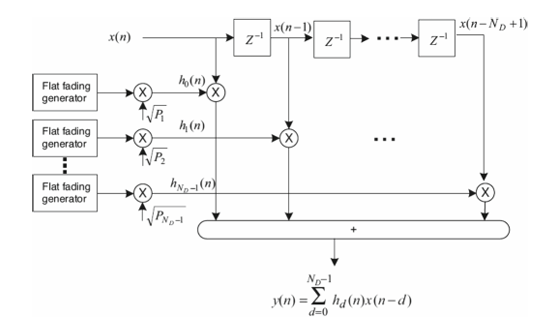
\includegraphics[width=1\textwidth]{schema1.png} 
        \caption{{ Fig.4. TDL}- based frequency selective fading channel model \textcolor{blue}[29]}
        \label{fig:example}
    \end{figure}



$N_{FFT}$, the sampling frequency or the sampling period which depends on the bandwidth, the OFDM symbol duration and the channel PDP. The frequency sampling is computed knowing the channel bandwidth $B$ Eq. \textcolor{blue}{ 13}\cite{31}. The symbol duration is computed based on the Eq. 10. As known, the sampling period is inversely proportional to the sampling frequency.

\begin{equation}
    F_s = \frac{64}{7} * \frac{B}{8}
\end{equation}
\begin{equation}
    T_u = \frac{N_{FFT}}{F_s}
\end{equation}
\begin{equation}
    T_s = \frac{1}{F_s}
\end{equation}

In order to make the tapped delays multiple of a sampling period, a tap adjustment based on a rounding method is applied. The channel characteristics (Root Mean Square (RMS) delay spread) are maintained when using this method. Furthermore, this method allows for preserving the number of paths and the power relative to each path. It consists in the shift of the tap into the closest sampling instance. Finally, a new tap delay $t_d'$ is obtained using Eq.12 \cite{30}.

\begin{equation}
    t_d' = \text{round}\left(\frac{t_d}{T_s} + 0.5\right) * T_s
\end{equation}

where $t_d$ is the tapped delays. Using this equation, the delay $t_d'$ becomes a multiple of a sampling period and is used in the channel modeling. Moreover, one can normalize the tapped delays in terms of number of subcarriers by canceling $T_s$ from this equation. $t_d'$ becomes a number without unit which is used to represent each tap when generating the channel impulse response.

The main steps of the channel modeling are summarized:
\begin{itemize}[label=-]
    \item Channel PDP definition including each path with its delay and its power.
     \item  Sampling period computation using the channel bandwidth and the number of subcarriers.
  \item  Paths delay positioning in terms of sample FFT using the rounding method.
   \item  Linear conversion of the path powers (fading) which is normally presented in dB.
   \item Paths power normalization.
    
    \item Generation of impulse response complex taps using a flat fading generator with Rayleigh distribution. This generator is modeled using two independent and identically-distributed Gaussian random variables with a zero mean and unit variance. These variables are defined using a built-in MATLAB function \texttt{randn}.
\end{itemize}





 

Due to this channel modeling method, one can generate several independent realisations of the channel. One hundred independent channel realisations are used in this work.

Furthermore, multipath propagation is characterized by means of RMS of the channel delays spread (Eq. \ref{eq:rms_delay_spread}). The RMS delay spread value should be limited to the guard interval (CP duration) to avoid ambiguities.

\begin{equation}
\tau_{\text{RMS}} = \sqrt{\frac{1}{\sum_{i=1}^{n}P_i} \cdot \sum_{i=1}^{n}( \tau_i^2 P_i) - \tau_d^2}
\quad \text{with} \quad \tau_d = \frac{\sum_{i=1}^{n} (\tau_i P_i)}{\sum_{i=1}^{n}P_i}
\label{eq:rms_delay_spread}
\end{equation}

\section*{4.3 Error Measurement Simulation Methodology}

As previously presented, the channel is generated using independent Gaussian distributed generators. In the receiver parameters, the resolution parameters for echoes are equal to 0.1 dB for the power and 10 ns for the delay. This means that for each echo value (path) the maximum uncertainty tolerable are $\pm10$ ns and $\pm0.1$ dB respectively for the delays and the powers measurement. To evaluate the impact of uncertainty error measurement on the channel, the following steps are processed.

\begin{itemize}[label=-]
    \item The channel flat fading generators are maintained non-random.
    \item Uncertainties about power, delay or both of them are randomly generated using a Gaussian distributed generator.
    \item Comparison of results to that obtained without uncertainty.
    \item Increase of power and delay uncertainties.
    \item Identification of the maximum uncertainty values for which the system performance could be considered negligible.
\end{itemize}

As 0.1 dB is considered to be the performance loss which could be considered as negligible at low BER, this criteria is used in this work.

\section*{4.4 System and Parameters}

In this part, light version of DVB-T2 system implemented is presented. It consists in the random generation of binary data which undergo LDPC coding,


%Finrosselin




\maketitle 
QAM mapping, OFDM and CP insertion processing. The signal obtained is convoluted with the channel impulse response. Uncertainties is added when generating the channel impulse response and the noise is added to the signal with channel effects. The reverse operations are performed at the receiver side. System performance is evaluated after channel equalization using MER and EVM and after LDPC decoder using BER. In the FBMC case study, CP-OFDM is substituted by FBMC. Table 4 presents the main parameters of DVB-T2 system. k is equal to 1024. The simulation parameters are presented in blue color. the channel bandwidth of 8 MHz is used as this is the most exploited in DVB-T2 implementation. As the subcarriers number used in this case is $8 \mathrm{k}=8192$, CFIR 1-tap equalizer is sufficient to perform demodulation. Also, when 8192 subcarriers are used in the native DVB-T2 system, $2 N_{F F T}$ subcarriers is applied in FBMC based DVB-T2 (Fig. 5).\\
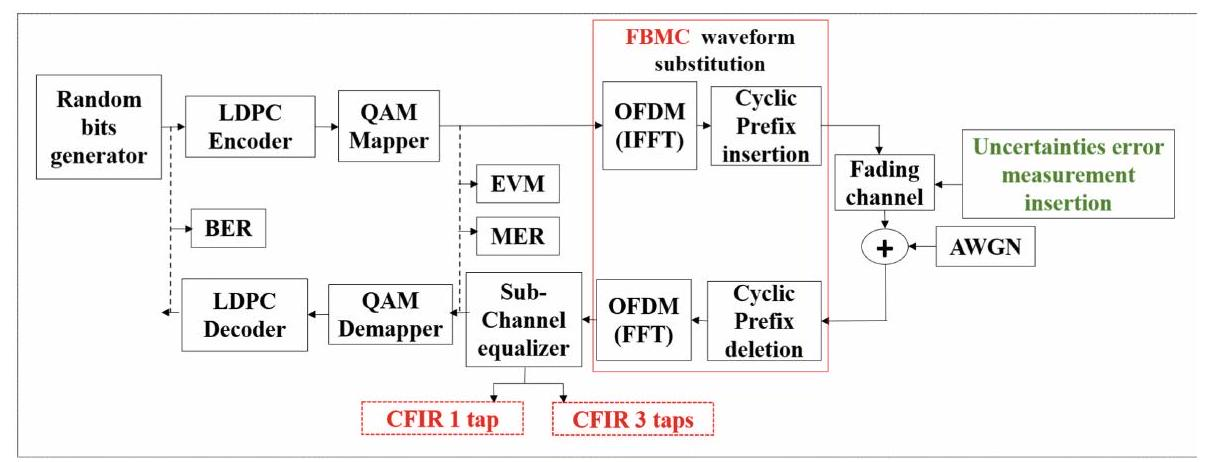
\includegraphics[max width=\textwidth, center]{2024_11_15_3776bfa3c020725d7730g-1}

Fig. 5. System implemented

Table 4. DVB-T2 systems parameters

\begin{center}
\begin{tabular}{l|l}
\hline
FFT mode & $1 \mathrm{k}, 2 \mathrm{k}, 4 \mathrm{k},((8,16,32) \mathrm{k}$ and ext) \\
\hline
Modulation & $4,16,64,256$-QAM \\
\hline
FEC frame & long $(64800$ bits), short (16200 bits) \\
\hline
Code Rate (CR) LDPC & $1 / 2,3 / 5,2 / 3,3 / 4,4 / 5,5 / 6$ \\
\hline
Bandwidth & $1.7,5,6,7,8,10 \mathrm{MHz}$ \\
\hline
CP & $1 / 128,1 / 32,1 / 16,19 / 256,1 / 8,19 / 128,1 / 4$ \\
\hline
\end{tabular}
\end{center}

In this section, simulation results obtained with uncertainty error measurement are presented. The mains performance evaluation tools used are BER, MER,

EVM and RMS delays spread. The channel RMS delay spread is equal to $2.810^{-7}$ s . This value is lower than the CP duration $\left(28.10^{-6} \mathrm{~s}\right)$. It changes with the variation of uncertainty values. The results are presented for both native DVBT2 system and DVB-T2 system based FBMC. This section is finalized by the discussion.\\
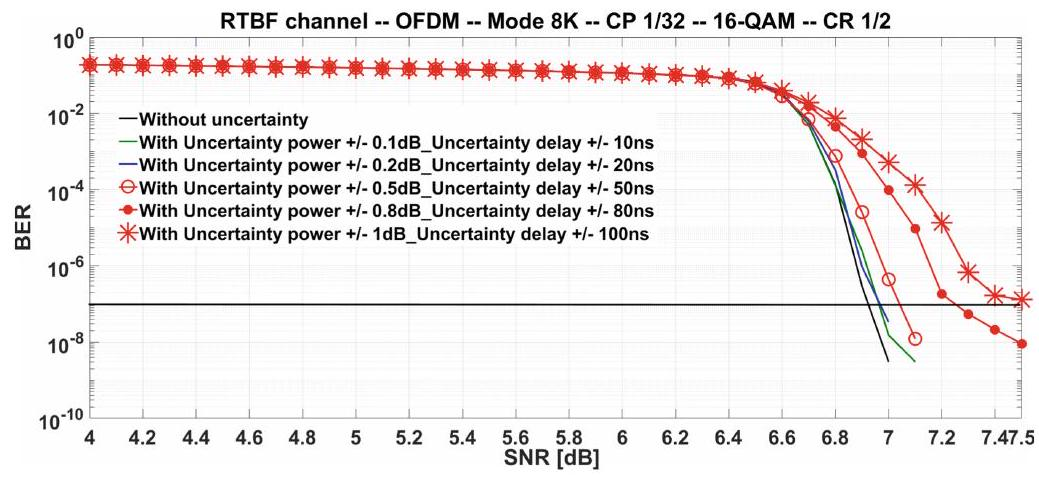
\includegraphics[max width=\textwidth, center]{2024_11_15_3776bfa3c020725d7730g-2}

Fig. 6. Impact of uncertainty error on OFDM based DVB-T2 system: BER

Table 5. Performance of DVB-T2 system in the presence of uncertainty error using RTBF channel

\begin{center}
\begin{tabular}{|c|c|c|c|c|c|c|}
\hline
\multicolumn{7}{|l|}{AWGN only} \\
\hline
\multicolumn{3}{|l|}{BER} & \multicolumn{4}{|l|}{SNR [dB]} \\
\hline
\multicolumn{3}{|l|}{$10^{-7}$} & \multicolumn{4}{|l|}{6.2 [29]} \\
\hline
\multicolumn{7}{|l|}{RTBF channel + AWGN} \\
\hline
- & - & $\pm 0.1$ dB & $\pm 0.2 \mathrm{~dB}$ & $\pm 0.5 \mathrm{~dB}$ & $\pm 0.8 \mathrm{~dB}$ & $\pm 1 \mathrm{~dB}$ \\
\hline
- & - & $\pm 10 \mathrm{~ns}$ & $\pm 20 \mathrm{~ns}$ & $\pm 50 \mathrm{~ns}$ & $\pm 80 \mathrm{~ns}$ & $\pm 100$ ns \\
\hline
BER & SNR [dB] & SNR [dB] & SNR [dB] & SNR [dB] & SNR [dB] & SNR [dB] \\
\hline
$10^{-7}$ & 6.92 & 6.96 & 6.96 & 7.05 & 7.26 & 7.5 \\
\hline
\multicolumn{7}{|l|}{Impact of fading channel and uncertainty} \\
\hline
- & Fading & \multicolumn{5}{|l|}{Impact of uncertainty} \\
\hline
BER & Loss [dB] & Loss [dB] & Loss [dB] & Loss [dB] & Loss [dB] & Loss [dB] \\
\hline
$10^{-7}$ & 0.81 & 0.04 & 0.04 & 0.13 & 0.34 & 0.58 \\
\hline
\end{tabular}
\end{center}

\subsection*{5.1 BER Evolution in Function of SNR}
\section*{1. Native DVB-T2 case (OFDM based DVB-T2)}
To validate the good behaviour of our simulator, simulation has been previously performed using only AWGN channel for both Native DVB-T2 and FBMC based DVB-T2 systems [14]. The results obtained have been compared to results presented in the guideline implementation using the same parameters [29]. Fading channel is applied in the system and non random fading generators are used to control the sole contribution of uncertainty variation. Figure 6 presents BER progression in function of SNR when the uncertainty error varies. Table 5 presents the results obtained at a BER of $10^{-7}$ and the loss obtained when compared to simulation without uncertainty. One can notice that when RTBF fading channel is used, the loss obtained is equal to 0.81 dB compared result with only AWGN. When equipment uncertainty ( 0.1 dB and 10 ns ) are inserted, the loss is equal to 0.04 dB . This value is negligible. However, when the uncertainty increases, the loss increases and becomes significant.

\section*{2. FBMC based DVB-T2 case}
When FBMC is applied in DVB-T2 instead OFDM, simulations have been performance when uncertainty values are not inserted and when uncertainty power values of $\pm 10 \mathrm{~ns}$ and 0.1 dB . Figure 7 depicts the results obtained at a BER of $10^{-7}$. One can noticed that the SNR values are similar in both cases (without and with uncertainties).\\
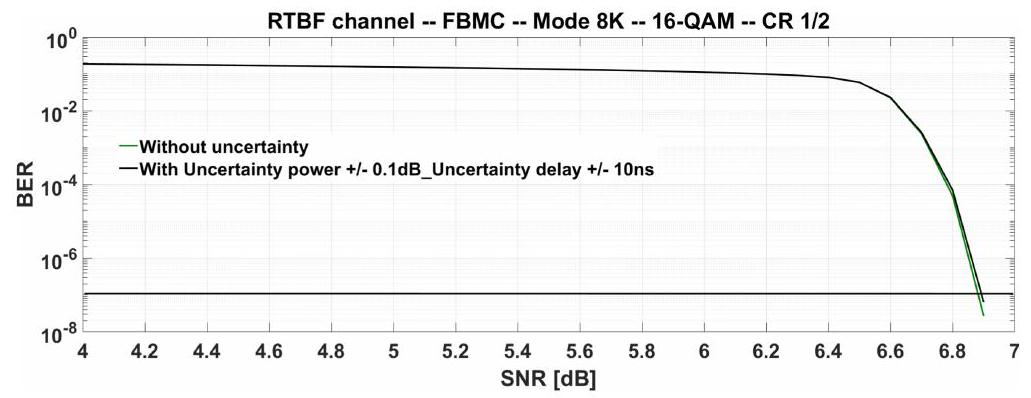
\includegraphics[max width=\textwidth, center]{2024_11_15_3776bfa3c020725d7730g-3}

Fig. 7. Impact of uncertainty error on FBMC based DVB-T2 system: BER

\subsection*{5.2 MER and EVM Evolution in Function of SNR}
\section*{1. Native DVB-T2 case}
As previously presented, MER is the tool used to measure the signal quality. In the case of the sole use of AWGN, MER is equal to SNR. When fading channel is used, MER value includes contribution of both AWGN and fading channel.\\
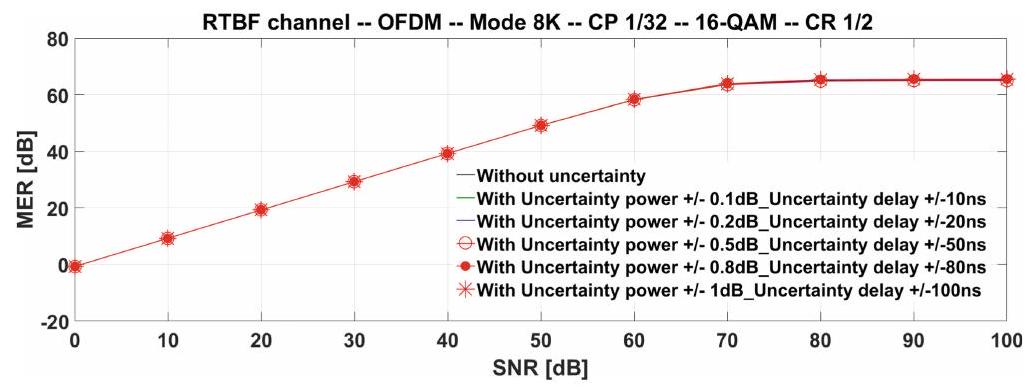
\includegraphics[max width=\textwidth, center]{2024_11_15_3776bfa3c020725d7730g-4}

Fig. 8. Impact of uncertainty error on OFDM based DVB-T2 system: MER

Figure 8 depicts MER progression in function of SNR. One can notice that the values of MER are comparable when uncertainties are applied or not. Also, these values are less than SNR values when fading channel is used. Furthermore, MER value is saturated for SNR higher than 65 dB . This means that even if the SNR increases, there is the residual effect of the channel which still remains in the received data. As previously presented, EVM is inversely proportional to MER. Figure 9 presents EVM evolution in function of SNR When OFDM is used. One can notice that the values of EVM are comparable when uncertainties are applied or not.

\section*{2. FBMC based DVB-T2 case}
Figure 10 presents MER and EVM evolution in function of SNR When FBMC is used instead of OFDM for all uncertainty value previously presented. One can note that there is no impact on the system performance in term MER and EVM when uncertainty value increases. Also, MER curve is saturated for SNR higher than 60 dB . This means that, compared to OFDM MER curve, there is the presence of the residual filter effects in the FBMC signal which decreases the MER values for high SNR values.\\
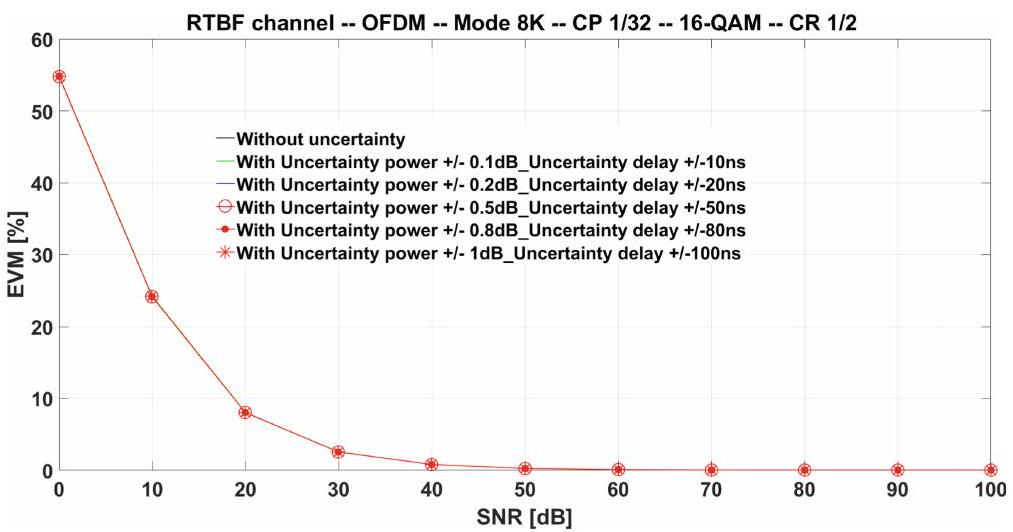
\includegraphics[max width=\textwidth, center]{2024_11_15_3776bfa3c020725d7730g-4(1)}

Fig. 9. Impact of uncertainty error on OFDM based DVB-T2 system: EVM

%debut_coincoin
\setcounter{page}{199}

\begin{figure}[h]
    \centering
    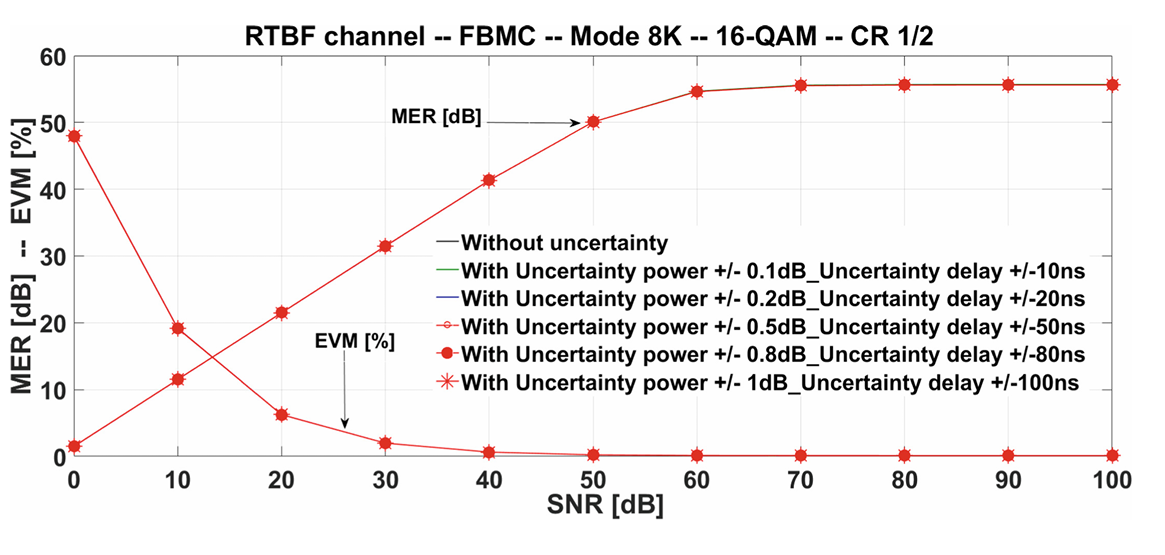
\includegraphics[width=\textwidth]{images/coicoin.png}
    \caption{\textbf{Fig. 10.} Impact of uncertainty error on FBMC based DVB-T2 system: MER and EVM}
\end{figure}

\section*{5.3 Discussion}

From all the results obtained, one can notice that the impact of channel uncertainty measurement in term of BER is negligible for normal measurement uncertainty values lower than 0.5 dB in power and lower than 50ns in delay in the case of the native DVB-T2 (CP-OFDM). When the uncertainties exceed these values the loss becomes significant (losses higher than 0.1 dB). In FBMC based DVB-T2 case, the impact is negligible in the normal reception condition (equipment uncertainty values: $\pm$0.1 dB in power and $\pm$10 ns in delay). Furthermore, the impact of uncertainty values is negligible in terms of MER and EVM for uncertainties range of powers 0.1 dB–1 dB and delays 50–100 ns. In order word, in this uncertainties range values, there is no impact on MER and EVM values. Also, the MER value expected for a rooftop antenna reception is at least 18 dB~\cite{Fisher}. In this MER range values, the impact of uncertainty is not noticeable. This work comes to fill the gap in research about the channel uncertainty measurement appear during the trials and the channel PDP recording. Also, it gives information details about a modified version of DVB-T2 (FBMC based DVB-T2) previously proposed in~\cite{Honfoga2019, Honfoga2020_1}. Besides DVB-T2 technology performance investigation during the last decade, Digital Audio Broadcasting plus (DAB+) technology is also a quite recent standard developed with the purpose to provide digital audio signal to receivers in fixed, portable and mobile reception scenarios. The analysis done in this work could be investigated in this standard to help broadcasters (in particular, in African countries) in the DAB+ network deployment.

\section*{6 Conclusion}

This work presents the simulation results and impact of channel uncertainty measurement on DVB-T2 and FBMC based DVB-T2 systems in terms of BER, MER and EVM. It shows that channel uncertainty measurement in power and delay is less impactful in FBMC based DVB-T2 for normal reception conditions, making it a more robust technology under varying measurement uncertainties.
However, the impact becomes relevant in term of BER for channel path powers greater than 0.5 dB and path delays greater than 50 ns for the native DVB-T2 system. This paper proves the range of uncertainty foreseen by the manufacturer and give details about the margin which can be exceeded by broadcasters during field and channel measurement. Also, it tackles the uncertainty range values predictable if FBMC was adopted like multicarrier modulation in the next generation of the European broadcasting standard. Furthermore, as most of European countries first deployed DVB-T system, the migration to DVB-T2 was effective in some countries where it still a challenge for other countries like Belgium. Indeed, the advent of 5G allows the development of 5G broadcast, it could provide audiovisual content to mobile receivers. Nevertheless, DVB-T2 presents many advantages against 5G broadcast and namely, the provision the rooftop antenna reception service which is not the specificity of 5G broadcast.

In perspectives, the work can be pursued as follows:

\begin{itemize}[label=-]
    \item Study of the impact of errors relative to the channel estimation in DVB-T2 system
    \item Study of impact of channel uncertainty measurement when MISO technique is applied in DVB-T2
    \item Evaluation of the impact of channel uncertainty during field measurement.
\end{itemize}

\begin{thebibliography}{99}

\bibitem{EBU2015_1}
European Broadcasting Union: Digital Video Broadcasting (DVB); Framing structure, channel coding and modulation for digital terrestrial television (DVB-T). DVB Document A012, June 2015.

\bibitem{Reitmeier}
Reitmeier, G.A., Smith, T.R.: An overview of the ATSC digital television standard. In: International Workshop on HDTV, Los Angeles, USA (1996). \href{https://doi.org/10.5594/M001266}{https://doi.org/10.5594/M001266}.

\bibitem{Takada}
Takada, M., Saito, M.: Transmission system for ISDB-T. Proc. IEEE 94(1), 251–256 (2006). \href{https://doi.org/10.1109/JPROC.2005.859692}{https://doi.org/10.1109/JPROC.2005.859692}.

\bibitem{Song2007}
Song, J., et al.: Technical review on Chinese digital terrestrial television broadcasting standard and measurements on some working modes. IEEE Trans. Broadcast. 53(1), 1–7 (2007). \href{https://doi.org/10.1109/TBC.2007.891835}{https://doi.org/10.1109/TBC.2007.891835}.

\bibitem{EBU2015_2}
European Broadcasting Union: Digital video broadcasting (DVB); Frame structure, channel coding and modulation for a second generation digital terrestrial television broadcasting systems (DVB-T2). ETSI EN 302 755 V1.4.1 (2015).

\bibitem{ATSC}
Advanced Television Systems Committee, ATSC Physical Layer Protocol: Next generation broadcasting system to handheld. Document A/322, Washington, January 2020.

\bibitem{Aragon}
Aragon-Zavala, A., Angeira, P., Montalban, J., Vargas-Rosales, C.: Radio propagation in terrestrial broadcasting television systems: a comprehensive survey. IEEE Access (2021). \href{https://doi.org/10.1109/ACCESS.2021.3061034}{https://doi.org/10.1109/ACCESS.2021.3061034}.

\bibitem{EBU2001}
European Broadcasting Union. Digital Video Broadcasting (DVB). Measurement guidelines for DVB systems. ETSI TR 101 290 V1.2.1. Recommendation (2001).

\bibitem{EBU2020}
European Broadcasting Union. Digital Video Broadcasting (DVB); Measurement guidelines for DVB systems. ETSI TR 101 290 V1.4.1. Recommendation (2020).

\bibitem{ITU2019_1}
International Telecommunication Union: Method for point-to-area predictions for terrestrial services in the frequency range 30 MHz to 4 000 MHz, UIT-R P.1546-6. Recommendation (2019).

\bibitem{ITU2019_2}
International Telecommunication Union: DVB-T coverage measurements and verification of planning criteria, UIT-R SM.1875-3. Recommendation (2019).

\bibitem{DVB}
Digital Video Broadcasting: DTT Deployment Data, DTT system choice map. DVB/EBU/BNE DTT Deployment Database. \href{https://dvb.org/solutions/dtt-deployment-data/}{https://dvb.org/solutions/dtt-deployment-data/}. Accessed 06 June 2021.

\bibitem{Bouvry}
Bouvry, D.: Impact de la répartition temporelle des composantes multi-trajets sur les performances de signaux DVB-T (Digital Video Broadcasting-Terrestrial), MSc thesis, UMONS/FPMs, in collaboration with Radio Television Belge Francophone, private communication, Belgium (2010).

\bibitem{Honfoga2019}
Honfoga, A.-C., Nguyen, T.T., Dossou, M., Moeyaert, V.: Application of FBMC to DVB-T2: a comparison vs classical OFDM transmissions. In: IEEE GlobalSIP Conference (2019). \href{https://doi.org/10.1109/GlobalSIP45357.2019.8969550}{https://doi.org/10.1109/GlobalSIP45357.2019.8969550}.

\bibitem{Honfoga2020_1}
Honfoga, A.-C., Dossou, M., Moeyaert, V.: Performance comparison of new waveforms applied to DVB-T2 transmissions. In: IEEE International Symposium on Broadband Multimedia Systems and Broadcasting (BMSB) (2020). \href{https://doi.org/10.1109/BMSB49480.2020.9379775}{https://doi.org/10.1109/BMSB49480.2020.9379775}.

\bibitem{Honfoga2020_2}
Honfoga, A.-C., Dossou, M., Dassi, P., Moeyaert, V. *Filtered-Based UFMC Waveform Applied on Joint DVB-T2/NUC System*. In: EAI AFRICOMM - 12th EAI International Conference on e-Infrastructure and e-Services for Developing Countries (2020). Available at:  
\url{https://doi.org/10.1007/978-3-030-70572-5_2}.


\bibitem{Schrieber}
Schrieber, F., Zoellner, J., Stadelmeier, L., Burow, R., Kattanek, F., Krueger, S.: Field trial of a redundancy on demand DVB-T2 system. In: IEEE International Symposium on Broadband Multimedia Systems and Broadcasting (BMSB) (2016). \href{https://doi.org/10.1109/BMSB.2016.7521909}{https://doi.org/10.1109/BMSB.2016.7521909}.

\bibitem{Jeon2016}
Jeon, S., Kim, S., Kim, J.-D., Yim, Z., Seo, J.-S.: Field trial results of 4K-UHD over DVB-T2 single frequency network in Republic of Korea. In: IEEE International Symposium on Broadband Multimedia Systems and Broadcasting (BMSB) (2016). \href{https://doi.org/10.1109/BMSB.2016.7522002}{https://doi.org/10.1109/BMSB.2016.7522002}.

\bibitem{Jeon2017}
Jeon, S., et al.: Preliminary field trial results for DVB-T2 indoor reception in Seoul: a single transmitter case. In: IEEE International Symposium on Broadband Multimedia Systems and Broadcasting (BMSB) (2017). \href{https://doi.org/10.1109/BMSB.2017.7986186}{https://doi.org/10.1109/BMSB.2017.7986186}.

\bibitem{Setiyanto}
Setiyanto, B., Hidayat, R., Mustika, I.W., Sunarno, S.: CNR and BER ranges for the DVB-T2 reception-success. Int. J. Electr. Comput. Eng. (IJECE) 7(6), 3727–3734 (2017). \href{https://doi.org/10.11591/ijece.v7i6.pp3727-3734}{https://doi.org/10.11591/ijece.v7i6.pp3727-3734}.

\bibitem{Iacob}
Iacob, M.I., Demciuc, Y.I., Avraam, I.A.: Comparative evaluation of received signal parameters in SFN DVB-T2 service area. In: Systems of Signal Synchronization, Generating and Processing in Telecommunications (SYNCHROINFO), Conference (2018). \href{https://doi.org/10.1109/SYNCHROINFO.2018.8456937}{https://doi.org/10.1109/SYNCHROINFO.2018.8456937}.

\bibitem{Fitriyani}
Fitriyani, D., Anwar, K., Saputri, D.M.: Study on radio frequency profile of Indonesia digital television DVB-T2 for urban areas. In: International Conference on Islam, Science, and Technology (ICONISTECH), Bandung, Indonesia (2019). \href{https://doi.org/10.4108/eai.11-7-2019.2297441}{https://doi.org/10.4108/eai.11-7-2019.2297441}.

\bibitem{Promwong}
Promwong, S., Tiengthong, T., Ruckveratham, B.: Measurement and modeling of DTTV–SFN propagation in Thailand. Wirel. Pers. Commun. 115(4), 2805–2818 (2020). \href{https://doi.org/10.1007/s11277-020-07533-6}{https://doi.org/10.1007/s11277-020-07533-6}.

\bibitem{Igbonoba}
Igbonoba, E.E.C., Omoifo, O.: Determination of DVB-T2 signal quality in Nigeria: a case study of Jos, Plateau State, Nigeria. Niger. J. Technol. 40, 81–88 (2021). \href{https://doi.org/10.4314/njt.v40i1.12}{https://doi.org/10.4314/njt.v40i1.12}.

\bibitem{Suwansukho}
Suwansukho, N., Promwong, S.: Evaluation of rotated constellation in DVB-T2 based on measurement data. In: 5th International Conference on Engineering, Applied Sciences and Technology (ICEAST), pp. 1–5 July (2019). \href{https://doi.org/10.1109/ICEAST.2019.8802572}{https://doi.org/10.1109/ICEAST.2019.8802572}.

\bibitem{Bellanger}
Bellanger, M. *FBMC Physical Layer: A Primer*. PHYDYAS, January 2010. Available at:  
\url{http://www.ict-phydyas.org/teamspace/internal-folder/FBMC-Primer_06-2010.pdf} (accessed 08 June 2021).


\bibitem{Louveaux}
Louveaux, J., et al.: Equalization and demodulation in the receiver (single antenna), PHYDYAS, July 2008. \href{http://www.ict-phydyas.org/delivrables/PHYDYAS-D3.1.pdf/view}{http://www.ict-phydyas.org/delivrables/PHYDYAS-D3.1.pdf/view}. Accessed 08 June 2021.

\bibitem{RohdeSchwarz}
Rohde \& Schwarz. *TV Test Receiver EFA, Models 40/43 (DVB-T)*. Available at:  
\url{https://scdn.rohde-schwarz.com/ur/pws/dl_downloads/dl_common_library/dl_brochures_and_datasheets/pdf1/EFA4x_text_datasheet.pdf} (accessed 08 June 2021).


\bibitem{EBU2012}
European Broadcasting Union, Digital Video Broadcasting (DVB); implementation guidelines for a second generation digital terrestrial television broadcasting system (DVB-T2). ETSI TS 102 831 V1.2.1, Recommendation (2012).

\bibitem{Cho}
Cho, Y.S., Kim, J., Yang, W.Y., Kang, C.G.: MIMO-OFDM Wireless Communications With Matlab. Wiley, Hoboken (2010). ISBN 9780470825631.

\bibitem{Fisher}
Fisher, W.: Digital Video and Audio Broadcasting Technology. Signals and Communication Technology, Springer, Heidelberg (2020). \href{https://doi.org/10.1007/978-3-030-32185-7}{https://doi.org/10.1007/978-3-030-32185-7}.

\end{thebibliography}

%fin_coincoin


\end{document}